%----------------------------------------------------------
% Fichier: rapport.tex    Auteur(s): Simon DÉSAULNIERS
% Date: 2013-04-28
%----------------------------------------------------------
% Rapport du Travail de Session du cours SMI1002 de
% l'Université du Québec à Trois-Rivières.
%----------------------------------------------------------
\documentclass[11pt,french]{article}

\usepackage[frenchb]{babel}
\usepackage[utf8]{inputenc}
\usepackage[T1]{fontenc}

\usepackage{graphicx}

\usepackage{hyperref}
\hypersetup{hidelinks}

% Style des pages
\usepackage{fancyhdr}
\pagestyle{fancy}
\lhead{Travail de Session}

% Caractères mathématiques
\usepackage{amssymb}

\usepackage{color}

\usepackage[final]{pdfpages}

% Affichage de code source
\usepackage{listings}
\definecolor{dkgreen}{rgb}{0,0.6,0}
\definecolor{dkblue}{rgb}{0,0,0.8}
\definecolor{gray}{rgb}{0.5,0.5,0.5}
\definecolor{mauve}{rgb}{0.58,0,0.82}

\usepackage{courier}

\lstset{ %
backgroundcolor=\color{white},   % choose the background color; you must add \usepackage{color} or \usepackage{xcolor}
basicstyle=\footnotesize,        % the size of the fonts that are used for the code
breakatwhitespace=false,         % sets if automatic breaks should only happen at whitespace
breaklines=true,                 % sets automatic line breaking
captionpos=b,                    % sets the caption-position to bottom
commentstyle=\color{dkblue},    % comment style
deletekeywords={...},            % if you want to delete keywords from the given language
escapeinside={\%*}{*)},          % if you want to add LaTeX within your code
extendedchars=true,              % lets you use non-ASCII characters; for 8-bits encodings only, does not work with UTF-8
frame=single,                    % adds a frame around the code
keywordstyle=\color{dkgreen},       % keyword style
morekeywords={*,...},            % if you want to add more keywords to the set
numbers=left,                    % where to put the line-numbers; possible values are (none, left, right)
numbersep=5pt,                   % how far the line-numbers are from the code
numberstyle=\tiny\color{gray}, % the style that is used for the line-numbers
rulecolor=\color{black},         % if not set, the frame-color may be changed on line-breaks within not-black text (e.g. comments (green here))
showspaces=false,                % show spaces everywhere adding particular underscores; it overrides 'showstringspaces'
showstringspaces=false,          % underline spaces within strings only
showtabs=false,                  % show tabs within strings adding particular underscores
stepnumber=2,                    % the step between two line-numbers. If it's 1, each line will be numbered
stringstyle=\color{red},     % string literal style
tabsize=2,                       % sets default tabsize to 2 spaces
xleftmargin=\parindent,
title=\lstname                   % show the filename of files included with \lstinputlisting; also try caption instead of title
}


\newcommand{\HRule}{\rule{\linewidth}{0.5mm}}


\begin{document}
    % PAGE TITRE
    \begin{titlepage}
        \begin{center}
    
            
\includegraphics[height=3cm]{./aux/bd1.png}
            \\[3cm]
            
            \textsc{\LARGE Base de Données II}
            \\[0.2cm]
            \textsc{\Large SMI1002}
            \\[2cm]
            \HRule \\[0.5cm]
            {\huge \bfseries Travail de Session}
            \HRule \\[2cm]
            Par\\
            Jordan Blanchette\\
            Simon Désaulniers\\
            Christophe Diamond\\
            Daniel St-Pierre

            \vfill
            2013-04-28\\
            Université du Québec à Trois-Rivières
            \thispagestyle{empty}
        \end{center}
    \end{titlepage}
    \newpage
    
    % TABLE DES MATIÈRES
    \pagenumbering{roman}
    \setcounter{page}{1}
    \tableofcontents
    \newpage

    % CORPS DU RAPPORT
    \pagenumbering{arabic}
    \setcounter{page}{1}

    \section*{Introduction} % (fold)
    \label{sec:Introduction}
        \subsection*{But} % (fold)
        \label{sub:but}
            Le Travail de session du cours SMI1002 vise à maîtriser la programmation d'une base
            de données avec gestion de la concurence de requêtes, l'élaboration de requêtes optimisées
            et la gestion de panne de matériel.
        % subsection but (end)
        \subsection*{Mise contexte} % (fold)
        \label{sub:mise-en-contexte}
            L'association LAN-UQTR a pour but d'organiser un événement annuel à l'UQTR destiné autant aux
            étudiants de l'UQTR que les résidents de la région de la mauricie et ses alentours. L'événement
            consiste en un rassemblement d'autour de 200 personnes dans une ou plusieurs salles à l'Université
            du Québec à Trois-Rivières pour une période de 48 heures. Les gens y participant apportent leur matériel
            informatique pour le brancher en réseau avec le reste des participants. Par la suite, ils jouent de façon
            libre avec les autres ou participent à différents tournois de jeux connus.\\

            L'organisation d'une telle activité nécessite de la préparation de quelques mois à l'avance afin de faire
            le plan des tournois organisés, les jeux disponibles et la liste des billets vendus. L'association LAN-UQTR
            a donc besoin d'un système informatique muni d'une base de données faisant la gestion du personnel, des joueurs,
            des équipes de jeux et des tournois lors de l'événement.
        % subsection mise-en-contexte (end)
    % section Introduction (end)
    \newpage

    \section{Conception UML} % (fold)
    \label{sec:concep-uml}
        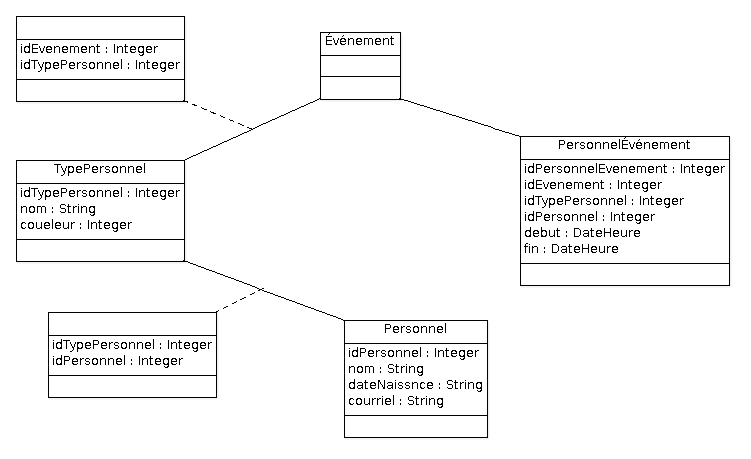
\includegraphics[width=12cm]{../../conception/conceptionBDevenement.png}

        problème avec les diagrammes... Y faudrait en faire d'autres (match pas avec la séparation des tâches qu'on vient de faire..)

        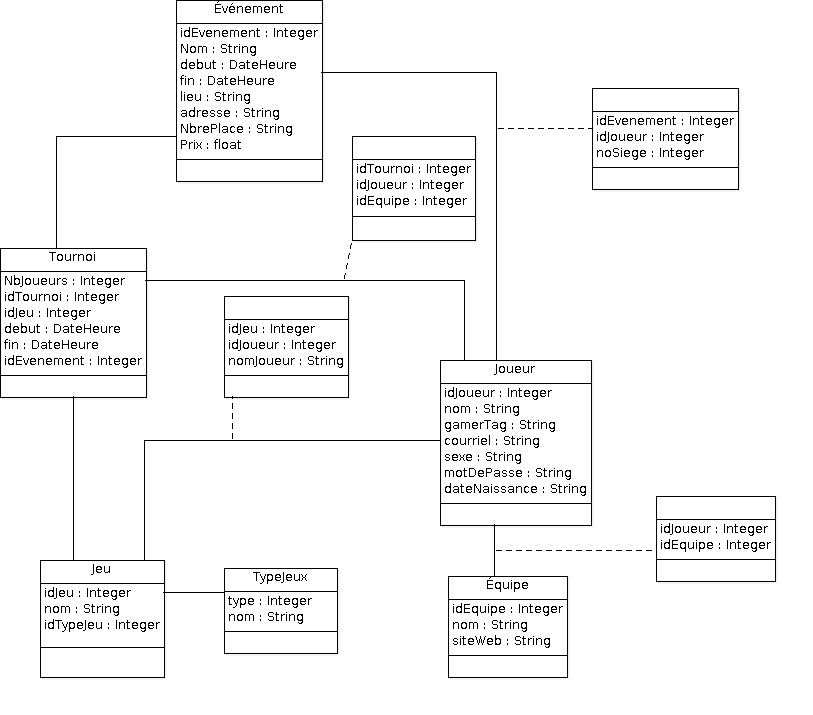
\includegraphics[height=12cm]{../../conception/conceptionBDpersonnel.png}
    % section concep-uml (end)
\end{document}
